\documentclass{webofc}
\usepackage[utf8]{inputenc}
\usepackage{xcolor}
\usepackage{minted}
\usepackage{tabto}
\usepackage{mathtools}
\usepackage{hyperref}

\title{Columnar data processing for HEP analysis}
\author{Jim Pivarski\inst{1} \and Jaydeep Nandi\inst{2} \and David Lange\inst{1} \and Peter Elmer\inst{1}}
\date{October 2018}

\abstract{In the last stages of data analysis, physicists are often forced to choose between simplicity and execution speed. In High Energy Physics (HEP), high-level languages like Python are known for ease of use but also very slow execution. However, Python is used in speed-critical data analysis in other fields of science and industry. In those fields, most operations are performed on Numpy arrays in an array programming style; this style can be adopted for HEP by introducing variable-sized, nested data structures. We describe how array programming may be extended for HEP use-cases and an implementation known as awkward-array. We also present integration with ROOT, Apache Arrow, and Parquet, as well as preliminary performance results.}

%% \abstract{In the last stages of data analysis, only order-of-magnitude computing speedups translate into increased human productivity, and only if they're not difficult to set up. Producing a plot in a second instead of an hour is life-changing, but not if it takes two hours to write the analysis code. Fortunately, HPC-inspired techniques can result in such large speedups, but unfortunately, they can be difficult to use in a HEP setting.

%% These techniques generally favor operating on columns— arrays representing a single attribute across events, rather than whole events individually— which allows data to stream predictably from disk media to main memory and finally to CPU/GPU/KNL onboard memory (e.g. L* cache) for prefetching and sometimes allows for for vectorization. However, the need to work with variable-length structures in HEP, such as different numbers of particles per event, makes it difficult to apply this technique to HEP problems.

%% We will describe several new software tools to make it easier to compute analysis functions with columnar arrays in HEP: array-at-a-time I/O in ROOT ("BulkIO") and Python/Numpy ("uproot"), compiling object-oriented analysis code into columnar operations ("oamap" for "object-array mapping"), and storage solutions with columnar granularity. We will show performance plots and usage examples.}

\xdefinecolor{dianablue}{rgb}{0.18,0.24,0.31}
\xdefinecolor{darkblue}{rgb}{0,0,1}
\xdefinecolor{darkgrey}{rgb}{0.35,0.35,0.35}
\xdefinecolor{darkorange}{rgb}{1.0,0.5,0}
\xdefinecolor{darkred}{rgb}{0.7,0,0}
\definecolor{darkgreen}{rgb}{0,0.5,0}
\definecolor{mauve}{rgb}{0.58,0,0.82}
\definecolor{lightviolet}{rgb}{0.65,0,1}

\definecolor{mycolor}{HTML}{FF6600}
\definecolor{cppcolor}{HTML}{00AAD4}
\definecolor{rootcolor}{HTML}{2A2AFF}
\definecolor{rootnpcolor}{HTML}{008000}
\definecolor{pythoncolor}{HTML}{FF00CC}

\begin{document}
\institute{Princeton University \and National Institute of Technology, Silchar, India}

\maketitle

\section{Introduction}

The field of High Energy Physics (HEP) has always dealt with big data, large enough datasets that finite memory and processing speed cannot be ignored. Traditionally, physicists have relied on compiled languages like Fortran and C++ to analyze large datasets in batch, but this limits interactive exploration. Today, data analysts in other academic fields and industry are developing tools to analyze large datasets in high-level languages, but these tools treat data as rectangular tables and flat arrays. HEP analysis requires {\it nested} data--- arbitrarily many tracks within jets or variable-sized collections of particle candidates--- which do not fit into rectangular data without padding and truncation.

This paper describes how the concepts of array programming may be extended to more complex data structures. It also introduces awkward-array~\cite{awkward}, an implementation of these ``awkward'' data structures as arrays, which is written in pure Python (depending only on Numpy~\cite{numpy}) for portability.

\section{Array programming and its extension to nested data}

Array programming is an interface in which individual user commands apply to whole arrays: each function call performs a regular operation on millions of data points. Pioneered by APL~\cite{apl} in 1962, this programming style appears primarily in analyst-facing data processing languages such as S~(1976), MATLAB~(1984), S-PLUS~(1988), R~(1993), and Numpy~(2005). Beyond its succinct syntax, which can be easier to read than the corresponding for loops, it encourages simple passes over columnar data that facilitates CPU cache-prefetching and vectorization. In fact, programs written in an array programming style are also appropriately organized for Single Instruction Multiple Data (SIMD) processing, which makes it easier to migrate to GPUs.

Array programming usually includes the following elements (expressed in Numpy syntax here):

\begin{description}
\item[\hspace{1 cm}$\bullet$] Multidimensional slices: \tabto{5.8 cm}{\small \mintinline{python}{rgb_pixels[0, 50:100, ::3]}}
\item[\hspace{1 cm}$\bullet$] Elementwise operations: \tabto{5.8 cm}{\small \mintinline{python}{all_pz = all_pt * sinh(all_eta)}}
\item[\hspace{1 cm}$\bullet$] Broadcasting: \tabto{5.8 cm}{\small \mintinline{python}{all_phi - 2*pi}}
\item[\hspace{1 cm}$\bullet$] Array reduction: \tabto{5.8 cm}{\small \mintinline{python}{array.sum()}} $\to$ scalar
\item[\hspace{1 cm}$\bullet$] Masking (list compaction): \tabto{5.8 cm}{\small \mintinline{python}{data[trigger & (pt > 40)]}}
\item[\hspace{1 cm}$\bullet$] Fancy indexing (``gather''): \tabto{5.8 cm}{\small \mintinline{python}{all_eta[argsort(all_pt)]}}
\item[\hspace{1 cm}$\bullet$] Row/column commutativity \tabto{5.8 cm}{\small \mintinline{python}{table["column"][7]} (row 7 of column array)}
\tabto{5.8 cm}{\small \mintinline{python}{table[7]["column"]} (field of row tuple 7)}
\end{description}

\noindent The semantics of each of these is well established for rectangular tables and flat arrays, but they can be extended to arbitrarily nested data structures. The examples below illustrate common cases that are defined in detail later in the text. In these examples, {\small\mintinline{python}{events["jets"]}}, {\small\mintinline{python}{jetpt}}, etc., contain lists of arbitrarily many objects or values.

\begin{description}
\item[\hspace{1 cm}$\bullet$] Multidimensional slices: \tabto{5.8 cm}{\small \mintinline{python}{events["jets"][:, 0]}} $\to$ first jet per event
\item[\hspace{1 cm}$\bullet$] Elementwise operations: \tabto{5.8 cm}{\small \mintinline{python}{jetpt * sinh(jeteta)}} $\to$ keep nested structure
\item[\hspace{1 cm}$\bullet$] Broadcasting: \tabto{5.8 cm}{\small \mintinline{python}{jetphi - metphi}} $\to$ expand {\small \mintinline{python}{metphi}} from
\tabto{5.8 cm}one-per-event to one-per-jet before operation
\item[\hspace{1 cm}$\bullet$] Array reduction: \tabto{5.8 cm}{\small \mintinline{python}{jetpt.max()}} $\to$ array of max jet $p_T$ per event
\item[\hspace{1 cm}$\bullet$] Masking (list compaction): \tabto{5.8 cm}{\small \mintinline{python}{data[trigger]}} $\to$ drop whole events
\tabto{5.8 cm}{\small \mintinline{python}{data[jetpt > 40]}} $\to$ drop jets from events  
\item[\hspace{1 cm}$\bullet$] Fancy indexing (``gather''): \tabto{5.8 cm}{\small \mintinline{python}{a = argmax(jetpt)}} $\to$ {\small \mintinline{python}{[[2], [], [1], [4]]}}
\tabto{5.8 cm}{\small \mintinline{python}{jeteta[a]}} $\to$ \mbox{\small \mintinline{python}{[[3.6], [], [-1.2], [0.4]]}\hspace{-0.5 cm}}
\item[\hspace{1 cm}$\bullet$] Row/column commutativity \tabto{5.8 cm}{\small \mintinline{python}{events["jets"]["pt"][7, 1]}} is the same as
\tabto{5.8 cm}{\small \mintinline{python}{events["jets"][7]["pt"][1]}} and \\
\tabto{5.8 cm}{\small \mintinline{python}{events["jets"][7, 1]["pt"]}} etc.
\end{description}

%% \noindent Consider the following extended example, which generates particle candidate combinations and then selects the best one. Procedural code like this (Python syntax):

%% {\small\begin{minted}{python}
%% leptoquarks = []
%% for event in dataset:
%%     best = None
%%     for jet in event.jets:
%%         for lepton in event.leptons:
%%             if cut(jet, lepton):
%%                 leptoquark = jet + lepton        # Lorentz vector + operator
%%                 if best is None or quality(leptoquark) > quality(best):
%%                     best = leptoquark
%%     if best is not None:
%%         leptoquarks.append(best)
%% \end{minted}
%% }

%% \noindent can be replaced by the following array-centric script.

%% {\small\begin{minted}{python}
%% pairs = events["jets"].cross(events["leptons"])  # cross-join within events
%% goodpairs = pairs[cut(pairs["0"], pairs["1"])]   # into pairs["0"] and ["1"]
%% candidates = pairs["0"] + pairs["1"]             # Lorentz vector + operator
%% best = candidates[quality(candidates).argmax()]  # best indexes, then objects
%% leptoquarks = best.flatten()                     # reduce to flat array
%% \end{minted}
%% }

\section{High-level types and array programming interface}

Arrays introduce a degree of static typing to dynamically typed programming languages, in the sense that all elements of an array have the same type and an operation only needs to perform a type-check once per array, rather than once per element. Conventional array processing environments like Numpy only support primitive types: numbers, booleans, and other fixed-size values (including records of fixed-size values). Fixed-size subarrays are presented as an array's multidimensional ``shape,'' and may be considered part of the type. Introducing nested data requires more data types. (Below, {\bf bold} keywords correspond to the bulleted lists of the previous section.)

The type of a flat array with length $n$ can be denoted $[0, n) \to P$, as a function signature that takes integers between $0$ (inclusive) and $n$ (exclusive) to a primitive type $P$. An array of length $n$ with variable-sized subarrays would be $[0, n) \to [0, \infty) \to P$, as any non-negative integer can be in the second domain. This is known as a jagged, or ragged, array. Jagged arrays may be nested: $[0, n) \to [0, \infty) \to [0, \infty) \to P$.

Extending the concept of {\bf multidimensional slices} from subintervals of $[0, n)$ to subintervals of $[0, \infty)$ is straightforward, though the result is itself jagged because some subarrays may be smaller than the slice and are clipped. {\bf Elementwise operations} also have a straightforward extension to jagged arrays, but not only must the total array lengths match among operands, their subarray lengths must match as well.

Conventional {\bf broadcasting} allows scalar $P$ data to be an operand in elementwise operations with arrays $[0, n) \to P$ by duplicating the one scalar to $n$ array elements. Jagged broadcasting duplicates each element of a flat array $[0, n) \to P$ to the corresponding jagged array elements $[0, n) \to [0, \infty) \to P$. The same applies for any depth of jaggedness: broadcasting increases the jaggedness of operands to match the jaggedness of the most deeply nested array.

{\bf Reducing} a flat $[0, n) \to P$ array, such as computing its sum, min, or max, returns a scalar $P$. Reducing a jagged $[0, n) \to [0, \infty) \to P$ array, such as computing the sum of each subarray, retuns $[0, n) \to P$, decreasing its jaggedness by one.

When {\bf masking} a jagged array, we may want to remove subarrays (representing events) or we may want to remove subarray elements (representing particles). We can make that distinction by contrasting a boolean mask $[0, n) \to \mbox{\small\tt bool}$ with a jagged boolean mask $[0, n) \to [0, \infty) \to \mbox{\small\tt bool}$. In keeping with the rules of conventional array programming, a boolean mask would remove subarrays from a jagged array $[0, n) \to [0, \infty) \to P$. Extending these rules, a jagged boolean mask can remove subarray elements if they have the same jagged structure.

Similarly, an integer array $[0, m) \to \mbox{\small\tt int}$ selects $m$ subarrays from a jagged array by the conventional rules, but a jagged integer array $[0, n) \to [0, \infty) \to \mbox{\small\tt int}$ can select subarray elements. Since this {\bf gather} feature is often used with functions like {\it argmax} and {\it argmin} to identify important indexes in one array and select elements at those indexes from another array, the jagged {\it argmax} and {\it argmin} should return jagged arrays with zero or one-element subarrays--- the max or min if any elements exist.

Tables with named, differently typed columns can be included in this type system as a mapping from names to types. For instance, a table with three columns is $[0, n) \to \{\mbox{\small\tt "one"} \to P_1\mbox{, }\mbox{\small\tt "two"} \to P_2\mbox{, }\mbox{\small\tt "three"} \to P_3\}$.

%% \[ [0, n) \to \left\{\begin{array}{l c l}
%% \mbox{\small\tt "one"} & \to & P_1 \\
%% \mbox{\small\tt "two"} & \to & P_2 \\
%% \mbox{\small\tt "three"} & \to & P_3\mbox{.} \end{array}\right. \]

In our extension of array programming, tables and jaggedness can be composed. This is useful in HEP for describing event records that contain variable-sized lists of particles, each with a different multiplicity, each containing attributes of various types. In some cases, it's useful for the particle attributes to be variable-sized lists as well. Type descriptions may then be arbitrary trees, like the following:

\vspace{-\baselineskip}
\[ [0, n) \to [0, \infty) \to \left\{\begin{array}{l c l}
\mbox{\small\tt "one"} & \to & [0, m) \to \left \{\begin{array}{l c l} \mbox{\small\tt "x"} & \to & [0, \infty) \to P_1 \\ \mbox{\small\tt "y"} & \to & P_2 \end{array}\right. \\
\mbox{\small\tt "two"} & \to & P_3 \\
\mbox{\small\tt "three"} & \to & P_4\mbox{.} \end{array}\right. \]

Rectangular tables can be sliced by row (integer index) or column (string index). So can jagged tables. A table described by $[0, n) \to [0, \infty) \to \{\mbox{\small\tt "one"} \to T_1\mbox{, }\mbox{\small\tt "two"} \to T_2\}$ sliced by a string index {\small\tt "one"} returns a jagged array $[0, n) \to [0, \infty) \to T_1$. In general, this means that integer indexes {\bf commute} with string indexes, though integer indexes do not commute with other integer indexes, nor do string indexes commute with other strings.

Primitives, variable-sized lists, and tables of records would be sufficient for most HEP cases, but sometimes polymorphic types and cross-references (pointers) are needed. Polymorphic types can be included with unions $T = T_1\ |\ T_2$ (elements may be type $T_1$ or type $T_2$) and optional types $?T$ (elements may be type $T$ or null). Since the possibilities of a polymorphic type are enumerated, operations must be legal on all enumerated possibilities, and operations on an optional type are only applied to non-null elements.

For cross-references, such as tagging jets with their associated leptons, we allow type trees to be arbitrary graphs. A list may contain elements of a list elsewhere in the graph or its own ancestors. As an example of the latter case,

\[ [0, n) \to T \coloneqq \big( \mbox{\small\tt int}\ \big|\ [0, \infty) \to T \big) \]

\noindent is an array that may contain integers, lists of integers, or any depth of lists of integers.

This set of types is as inclusive as most high-level programming languages, and it can be constructed entirely from columnar arrays.

\section{Low-level data structures and their uses}

The fundamental construct for variable-sized, nested structure is the jagged array. To represent a list of unequal-length sublists with the following logical structure, we store the flattened content in one array and the structure in either an ``offsets'' or a ``parents'' array.

\vspace{\baselineskip}
Logical structure: \tabto{4 cm}{\ttfamily\textcolor{black}{[\textcolor{red}{[}\textcolor{darkblue}{0, 1, 2}], \textcolor{red}{[}], \textcolor{red}{[}\textcolor{darkblue}{3, 4}], \textcolor{red}{[}\textcolor{darkblue}{5, 6, 7, 8}], \textcolor{red}{[}]\ \ \textcolor{red}{]}}}

\vspace{0.05 cm}
Content:           \tabto{4 cm}{\ttfamily\verb|[ |\textcolor{darkblue}{0, 1, 2}\verb|,       |\textcolor{darkblue}{3, 4}\verb|,   |\textcolor{darkblue}{5, 6, 7, 8}\verb|]|}

\vspace{0.05 cm}
Offsets:           \tabto{4 cm}{\ttfamily\verb|[|\textcolor{red}{0,}\verb|         |\textcolor{red}{3,}\verb|  |\textcolor{red}{3,}\verb|      |\textcolor{red}{5,}\verb|            |\textcolor{red}{10, 10}\verb|]|}

\vspace{0.05 cm}
Parents:           \tabto{4 cm}{\ttfamily\verb|[ |\textcolor{darkgreen}{0, 0, 0}\verb|        |\textcolor{lightviolet}{2, 2,}\verb|   |\textcolor{darkorange}{3, 3, 3, 3}\verb|]|}

\vspace{\baselineskip}
The offsets array may be constructed as the content index after every opening bracket (the ``starts'' array) appended by the total length, or it may be constructed as the content index after every closing bracket (the ``stops'' array) prepended by zero. It is useful for descending from outer levels to inner levels of structure.

The parents array has the same length as the contents array; it associates each content element with the index of the subarray that contains it. A parents array is incapable of expressing empty sublists at the end of a list (as in the above example), but it can specify empty lists in a sequence by skipping integers. Offsets are therefore more general than parents, but parents are useful in reducer operations that ascend from inner levels to outer levels of structure. 

The awkward-array library has a {\tt\small JaggedArray} implementation that allows arbitrary contents--- nesting a {\tt\small JaggedArray} within a {\tt\small JaggedArray} constructs $[0, n) \to [0, \infty) \to [0, \infty) \to P$. The {\tt\small JaggedArray.\_\_getitem\_\_} method overrides square brackets in Python to provide slicing, masking, and fancy indexing with all the features described in the previous section. Elementwise operations and broadcasting are implemented in {\tt\small \_\_array\_ufunc\_\_}, which overrides the behavior of all universal functions in Numpy~\cite{nep13}.

Tables of records are implemented as a {\tt\small Table} class that maps column names to arrays. This is like Numpy's ``record arrays,'' except that a Numpy record array must be a contiguous array of structs, while awkward-array's {\tt\small Table} may be non-contiguous or a struct of arrays. {\tt\small JaggedArray} and {\tt\small Table} interact to let integer and string valued indexes commute, which hides the arrays-of-structs/structs-of-arrays distinction.

{\tt\small UnionArray} and {\tt\small MaskedArray} implement polymorphism and optional types. Numpy has a masked array type, but {\tt\small MaskedArray} shares conventions with the rest of awkward-array's suite and additionally has a {\tt\small BitMaskedArray} variant for compatibility with Apache Arrow~\cite{arrow} (next section).

In HEP applications, it is useful to have datasets representing arrays of objects, such as $[0, n) \to \mbox{\tt\small LorentzVector}$, which returns \mbox{\tt\small LorentzVector} objects when given an index. Numpy has an ``object array'' type, which stores pointers to Python objects in memory, but awkward-array's {\tt\small ObjectArray} constructs a Python object when given an index. This allows us to represent such data with 12$\times$ less memory, as we will see in the section on performance below.

In the same spirit as integer/string index commutivity, methods of objects returned by {\tt\small ObjectArray} may be applied to the entire array for vectorized HEP calculations. For instance, an {\tt\small ObjectArray} of \mbox{\tt\small LorentzVectors} may be boosted en masse:

\begin{center}
\tt\small subleading\_jets.boost(leading\_jets)
\end{center}

\noindent which works equally well if {\tt\small subleading\_jets} is a jagged array (several per event) and {\tt\small leading\_jets} is a flat array (one per event), thanks to jagged broadcasting. An array of strings is an {\tt\small ObjectArray} of a {\tt\small JaggedArray}, converting subarrays of characters into {\tt\small str} objects on demand.

In addition, awkward-array provides some array classes for dealing with data structures without affecting their high-level data types. Some file formats provide data in discontiguous chunks, such as ROOT's baskets~\cite{root-file} or Parquet's pages and row groups~\cite{parquet-file}. {\tt\small ChunkedArray} lets us view discontiguous chunks of data as a single logical array without copying. {\tt\small VirtualArray} uses a given function to generate an array on demand, rather than holding it in memory (optionally passing it to a temporary cache). A chunked, virtual array corresponds to Dask's concept of a delayed array~\cite{dask}.

Any of these can be cross-referenced in Python, as the implementation is careful to avoid infinite recursion. To cross-reference array elements, to associate a single lepton with a jet for instance, {\tt\small IndexedArray} represents a deferred indirection. An {\tt\small index} array stores locations {\tt\small j[i]} to look up in a {\tt\small content} array: given {\tt\small i}, it returns {\tt\small content[j[i]]}. {\tt\small JaggedArray} is like {\tt\small IndexedArray} except that it represents ranges of {\tt\small content} indexes, rather than individual indexes.

{\tt\small SparseArray} is the conceptual opposite of {\tt\small IndexedArray}: its {\tt\small index} and {\tt\small content} must be the same length and each {\tt\small index} is the logical position of the corresponding {\tt\small content}. Other indexes are presumed to be zero or some default value. As a sparse matrix, this is known as the COOrdinate format~\cite{coo}. Whereas an {\tt\small IndexedArray} represents a smaller logical array than its {\tt\small content} (or one with duplicates), a {\tt\small SparseArray} represents a larger logical array than its {\tt\small content}. It is useful in HEP for looking up indexes in a table that is far too large to fit in memory, such as a mapping from ten-digit detector id numbers to measurement corrections.

\section{ROOT/Arrow/Parquet compatibility and persistence}

The awkward-array classes were not designed to be a new format, but to give existing formats new behaviors, so that they can be used in an array programming style. As such, they are configurable to fit a variety of representations. %% For instance, there are six ways to configure {\tt\small MaskedArrays}: the mask may be bytes, bits, ``true means masked'' or ``false means masked,'' and if bits, the order may be least significant bit first or most significant bit first. Numpy's masked arrays use bytes in which ``true means masked'' and Arrow's arrays (all of which are masked) use bits in which ``false means masked'' in least significant bit order (opposite of Numpy's {\it packbits}).

The scope of awkward-array was chosen such that ROOT, Apache Arrow, and Parquet data may be viewed through configurations of the awkward classes. Numpy natively supports the full range of numeric types, big and little endian byte orders, and fixed-size subarrays, which awkward-array inherits. {\tt\small ByteJaggedArray} can use ROOT's basket format directly, which specifies the positions of variable-sized entries by byte index. All the baskets in a branch may be viewed as a {\tt\small ChunkedArray}, while lazy loading and decompression are provided by {\tt\small VirtualArray}. A ROOT TTree is a (possibly jagged) {\tt\small Table}, and pointer references can be emulated with {\tt\small IndexedArray}. Arbitrary C++ types are encoded in ROOT's streamers, which uproot~\cite{uproot} translates to Python classes. Data with this general type are then presented as {\tt\small ObjectArrays} with {\tt\small TLorentzVector} being the primary example.

Apache Arrow has a simpler data model consisting only of primitives, arbitrary-length lists, records, unions, strings, date/time types, and ``dictionary encodings,'' in which a small set of large values, such as the names of categories (strings), are represented by fixed-width integers for efficiency. All of these arrays are bit-masked to allow missing (null) data anywhere. {\tt\small JaggedArrays} represent the lists, {\tt\small Tables} the records, {\tt\small UnionArrays} the unions, {\tt\small StringArrays} (which are just {\tt\small JaggedArrays} of characters) represent the strings, and {\tt\small ObjectArrays} represent the date/time types. Dictionary encodings are {\tt\small IndexedArrays} without cross-references. The Parquet file format is wildly different, beyond the scope of awkward-array to wrap directly, but pyarrow (the Python front-end for Arrow-C++ and Parquet-C++) converts Parquet into Arrow.

Although most data would be drawn from a standard format like ROOT (in HEP) or Parquet (beyond HEP), it is often necessary to save derived quantities after some analysis. Derived quantities might use features not available in the source format. Therefore, awkward-array has its own persistence format: a JSON string describing how awkward-array classes are nested with cross-references and a binary blob for each array. These may be placed in any container of named binary blobs, such as a ZIP file, an HDF5 file, or a distributed object store. By default, {\tt\small VirtualArrays} representing data from ROOT or Parquet are saved as instructions for reading from the original file, rather than the data themselves. Thus, an analyst can read ROOT or Parquet data, add or replace fields in its {\tt\small Tables}, and save the ensemble in a file representing only the changes, which can be considerably smaller than the original data.

%% The JSON description of the awkward-array structure is formatted like an executable LISP expression, providing a high degree of forward compatibility: later versions may construct new expressions, but they are executable in older versions of the awkward-array library. The deserialization process checks function names against a whitelist of allowed functions for security. Python values are expressed in JSON for cross-language compatibility as much as possible, though pickle is a fallback.

\section{Performance measurements}

The data structures and operations described here were designed for performance, but a full study has not yet been carried out. Such a study would require a target HEP analysis, since performance differs in detail from one analysis to the next. However, arrays have a natural order parameter: their size, which should be chosen to significantly exceed any metadata in the awkward-array classes. It also has an obvious hotspot: stepping through Python instructions is significantly slower than any numerical operations. This prescribes a simple rule--- Python code should never iterate over all elements of an array; any operation that scales with the number of elements in an array must be performed in compiled code (i.e.\ Numpy).

As a rough indicator of performance trade-offs, we studied one operation in a variety of contexts, the jagged elementwise calculation
\begin{center}
\mintinline{python}{pz = pt * numpy.sinh(eta)}
\end{center}
\noindent where \mintinline{python}{pt} and \mintinline{python}{eta} are jagged arrays with the same structure: 552,056 muons in 701,716 events. These tests were performed on CERN's SWAN service and all files to reproduce the study are shared publicly on CERNBox~\cite{performance}. Table~\ref{quantify} shows the memory used to store these data before calculation and the time to compute in awkward-array, ROOT, pure Python, and instrumented Python like awkward-array and PyROOT in which Python code is iterating over all elements of the arrays. The differences span orders of magnitude.

\begin{table}
\caption{Horizontal study of \mintinline{python}{pz = pt * numpy.sinh(eta)} in many types of systems. \label{quantify}}

\begin{minipage}{0.4\linewidth}\scriptsize
\begin{tabular}{r p{0.9\linewidth}}
\underline{MB} & \underline{RAM memory occupied by data} \\
& \\
311.95 & \textcolor{pythoncolor}{Python list of lists of dicts} \\
215.11 & \textcolor{rootnpcolor}{root\_numpy's array of arrays} \\
139.79 & \textcolor{pythoncolor}{Python list of lists of {\tt \_\_slots\_\_} classes} \\
& \\
 37.19 & \textcolor{gray}{serialized JSON text} \\
& \\
 22.38 & \textcolor{cppcolor}{{\tt\scriptsize std::vector<std::vector<struct>>}} \\
& \\
 11.67 & \textcolor{mycolor}{JaggedArray of Table of pt, eta, phi} \\
%% & \\
%% & \textcolor{gray}{\scriptsize 1 MB = 1024$^2$ bytes} \\
%% & \textcolor{gray}{\scriptsize 701,716 events containing 552,056 muons} \\
%% & \textcolor{gray}{\scriptsize storing pt, eta, phi as float32} \\
\end{tabular}

\vspace{1.35 cm}
\end{minipage}\begin{minipage}{0.6\linewidth}{\mbox{\hspace{-3.5 cm}\begin{minipage}{1.5\linewidth}\scriptsize
\begin{tabular}{p{0.83\linewidth} l}
\hfill \underline{time to complete load, compute, or both} & \underline{sec} \\
& \\
\hfill \textcolor{rootcolor}{PyROOT load and compute} & 45.9 \\
\hfill \textcolor{mycolor}{JaggedArray compute in Python for loops} & 13.4 \\
& \\
\hfill \textcolor{rootnpcolor}{root\_numpy compute in loop over ufuncs} & \ 1.96 \\
\hfill \textcolor{pythoncolor}{Python list of lists of dicts in Python for loops} & \ 1.24 \\
\hfill \textcolor{pythoncolor}{Python list of lists of {\tt \_\_slots\_\_} classes in Python for loops} & \ 1.23 \\
\hfill \textcolor{rootnpcolor}{root\_numpy load} & \ 0.635 \\
& \\
\hfill \textcolor{rootcolor}{ROOT RDataFrame load and compute} & \ 0.163 \\          % -O0: 0.326, -O1: 0.172, -O2: 0.162, -O3: 0.163
\hfill \textcolor{rootcolor}{ROOT TTreeReader load and compute} &  \ 0.091 \\        % -O0: 0.164, -O1: 0.071, -O2: 0.091, -O3: 0.091
\hfill \textcolor{rootcolor}{ROOT TBranch::GetEntry load and compute} & \ 0.046 \\   % -O0: 0.052, -O1: 0.049, -O2: 0.049, -O3: 0.046
\hfill \textcolor{mycolor}{uproot load} & \ 0.031 \\
\hfill \textcolor{mycolor}{JaggedArray compute as Numpy-like ufunc} & \ 0.023 \\
\hfill \textcolor{mycolor}{JaggedArray compute in Numba-accelerated Python for loops} & \ 0.023 \\
%% & \\
%% \hfill \textcolor{gray}{\scriptsize all with warmed disk cache in the same environment} & \\
\end{tabular}
\end{minipage}}}\end{minipage}
\end{table}

If this style of programming is adopted for HEP analysis, it presents an opportunity to optimize the array primitives independently of the analysis code. Array-centric data structures are ripe for vectorization, but some of the na\"ive algorithms, such as jagged reduction, have loop-carried dependencies that prevent vectorization. One of us (Nandi) developed vectorized algorithms for jagged operations~\cite{jaydeep}, such as this CUDA implementation of jagged reduction (fully described in a notebook~\cite{performance2}):
\begin{center}
\begin{minipage}{0.7\linewidth}
{\small\begin{minted}{python}
int i = threadIdx.x;
for (int d = 1;  d < blockSize.x;  d *= 2) {
    if (i >= d  &&  parents[i] == parents[i - d]) {
        content[i] += content[i - d];
    }
    __syncthreads();
}
\end{minted}
}
\end{minipage}
\end{center}
\noindent The rate of this algorithm on a Tesla P100 GPU and vector instructions on a Xeon Silver 4110 CPU are shown in Figure~\ref{rates_logy} as a function of the Poisson average number of items per group. For comparison, two sequential algorithms (nested for loops with all compiler optimizations, same CPU) are overlaid.

\begin{figure}[bh]
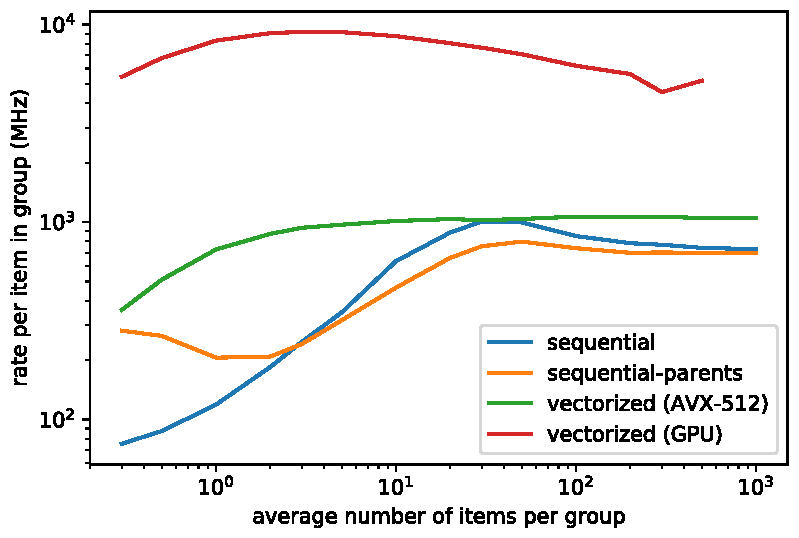
\includegraphics[width=0.48\linewidth]{sum_rates_logy.pdf}\hfill 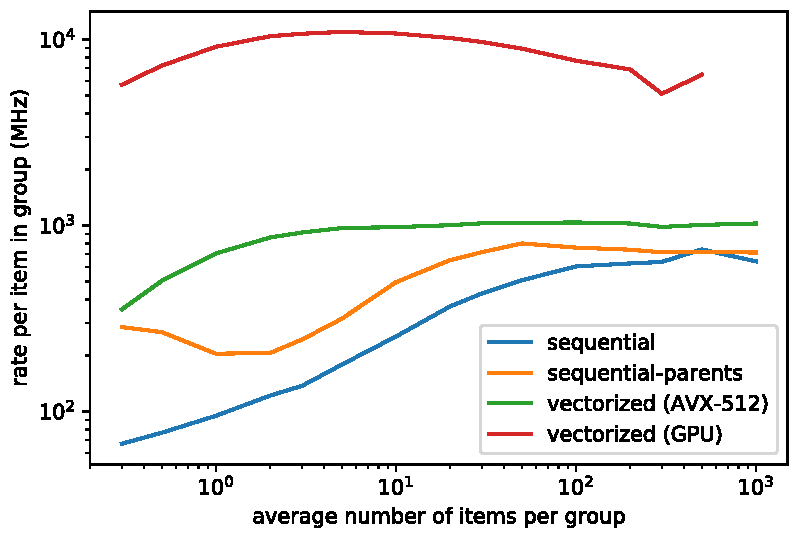
\includegraphics[width=0.48\linewidth]{max_rates_logy.pdf}

\caption{Jagged reduction \mintinline{python}{jaggedarray.sum()} (left) and \mintinline{python}{jaggedarray.max()} (right) for two sequential algorithms (CPU) and our vectorized algorithm on CPU and GPU. \label{rates_logy}}
\vspace{-0.5 cm}
\end{figure}

\section{Future directions}

Numpy arrays are the common language of Python's scientific ecosystem. Now that structures necessary for HEP have been cast as arrays, they can be more easily integrated into this ecosystem. As a next step, awkward-arrays will be added as a Pandas~\cite{pandas} extension type, so that columns in a Pandas DataFrame may be structured. Following that, {\tt\small ChunkedArrays} of {\tt\small VirtualArrays} will be wrapped as Dask delayed arrays so that calculations can be distributed without moving data. Problems that require conventional loops and conditionals can be optimized by wrapping awkward-arrays as Numba extensions. Finally, awkward-array's exclusive dependence on Numpy should make it transparently portable to GPUs with CuPy~\cite{cupy}, but that remains to be tested.

\section{Acknowledgements}

This work was supported by the National Science Foundation under grants ACI-1450377 and PHY-1624356.

\begin{thebibliography}{8}
% Journal Author, Journal \textbf{Volume}, page numbers (year)

\bibitem{awkward} Jim Pivarski, ``awkward-array'' [software], Release 0.4.1, Zenodo, 26 October, 2018. \textcolor{blue}{\url{https://zenodo.org/record/1472437}}

\bibitem{numpy} Travis E, Oliphant, ``A guide to NumPy,'' USA: Trelgol Publishing, (2006).

\bibitem{apl} Kenneth E.\ Iverson, \textit{A programming language} (John Wiley \& Sons, Inc., New York, 1962).

\bibitem{nep13} Blake Griffith, ``NEP 13: a mechanism for overriding ufuncs'' [Numpy Enhancement Proposal (accepted)], 10 July 2017. \textcolor{blue}{\url{https://www.numpy.org/neps/nep-0013-ufunc-overrides.html}}

\bibitem{arrow} Arrow Development Team, ``Apache Arrow'' [website]. \textcolor{blue}{\url{https://arrow.apache.org}}

\bibitem{root-file} Rene Brun and Fons Rademakers, ``The ROOT Object I/O System'' [specification], 26 August, 1996. \textcolor{blue}{\url{https://root.cern.ch/root/InputOutput.html}}

\bibitem{parquet-file} Julien Le Dem, ``Apache Parquet'' [specification], 29 April 2015. \textcolor{blue}{\url{https://parquet.apache.org/documentation/latest}}

\bibitem{dask} Dask Development Team, ``Dask: Library for dynamic task scheduling'' 2016. \textcolor{blue}{\url{https://dask.org}}

\bibitem{coo} Youcef Saad, ``SPARSKIT: a basic tool kit for sparse matrix computations'' [technical report], 21 May 1990. \textcolor{blue}{\url{https://ntrs.nasa.gov/search.jsp?R=19910023551}}

\bibitem{uproot} Jim Pivarski et al., ``uproot'' [software], Release 3.2.6, Zenodo, 22 October, 2018. \textcolor{blue}{\url{https://zenodo.org/record/1469102}}

\bibitem{performance} Performance test 1: \textcolor{blue}{\url{https://cernbox.cern.ch/index.php/s/uhAH75uGCddFlFL}}

\bibitem{jaydeep} Jaydeep Nandi, ``Vectorized proof of concepts'' [notebooks] August 2018. \\ \textcolor{blue}{\url{https://gitlab.com/Jayd_1234/GSoC_vectorized_proof_of_concepts}}

\bibitem{performance2} Performance test 2: \textcolor{blue}{\url{https://github.com/jpivarski/jupyter-performance-studies/blob/master/2018-09-10-jagged-reduction.ipynb}}

\bibitem{pandas} Wes McKinney, ``Data Structures for Statistical Computing in Python,'' Proceedings of the 9th Python in Science Conference, 51-56 (2010) (\textcolor{blue}{\href{http://conference.scipy.org/proceedings/scipy2010/mckinney.html}{publisher link}}).

\bibitem{cupy} Ryosuke Okuta, Yuya Unno, Daisuke Nishino, Shohei Hido and Crissman Loomis, ``CuPy: A NumPy-Compatible Library for NVIDIA GPU Calculations.'' Proceedings of Workshop on Machine Learning Systems (LearningSys), 31$^{\mbox{\scriptsize st}}$ Annual Conference on Neural Information Processing Systems (NIPS), (2017) (\textcolor{blue}{\href{http://learningsys.org/nips17/assets/papers/paper_16.pdf}{publisher link}}).

\end{thebibliography}

\end{document}
